\chapter{Implementación y pruebas}
\section{SCRUM}
\subsection{Product Backlog}
\begin{table}[h!]
	\centering
	\begin{tabular}{lcc}
		\toprule
		\textbf{Historia de Usuario} & \textbf{Estimación} & \textbf{Prioridad} \\
		\midrule
		Como usuario quiero poder identificarme en el sistema.	& 2	& 1 \\
		Como usuario quiero poder añadir otros usuarios en el sistema. & 2 &2 \\
		Como usuario quiero poder añadir alumnos al listado. & 1 & 3 \\
		Como usuario quiero poder buscar y seleccionar alumnos entre el listado. & 1 & 4 \\
		Como usuario quiero poder visualizar un listado de alumnos. & 3 & 5 \\
		Como usuario me interesa poder guardar los datos almacenados externamente. & 2 &6 \\
		Como usuario me interesa poder cargar los datos almacenados externamente. & 2 & 7 \\
		Como usuario quiero poder modificar alumnos del listado. &	1&	8 \\
		Como usuario quiero poder eliminar alumnos del listado.	 & 1 &	9 \\
		\bottomrule
\end{tabular}
\caption{\label{tab:product_backlog}Product Backlog}
\end{table}

\newpage
\subsection{Sprint Backlog}
\begin{table}[h!]
	\centering
	\begin{tabular}{cccccc}
		\toprule
		\textbf{Tarea} & \textbf{Quién} & \textbf{Estado} & \textbf{Semana 1} & \textbf{Semana 2} & \textbf{Semana 3} \\
		\midrule
		HU008.	& i72pehej & Terminada & 0.5 & 0.5 & 0 \\
		HU009.	& i72pehej & Terminada & 0.5 & 0.5 & 0 \\
		HU001.	& i72orled & Terminada & 0.5 & 0 & 0 \\
		HU004.	& i42semoa & Terminada & 0.5 & 0 & 0 \\
		HU005.	& i42semoa & Terminada & 4 & 2 & 0 \\
		HU006.	& i72pehej & Terminada & 2 & 1 & 0 \\
		HU007.	& i72pehej & Terminada & 2 & 1 & 0 \\
		HU002.	& i72orled & Terminada & 1 & 0.5 & 0 \\
		HU003.	& i72orled & Terminada & 1 & 0 & 0 \\
		\bottomrule
\end{tabular}
\caption{\label{tab:sprint_backlog}Sprint Backlog}
\end{table}

\subsection{Burndown Chart}
\begin{figure}[h!]
	\centering
	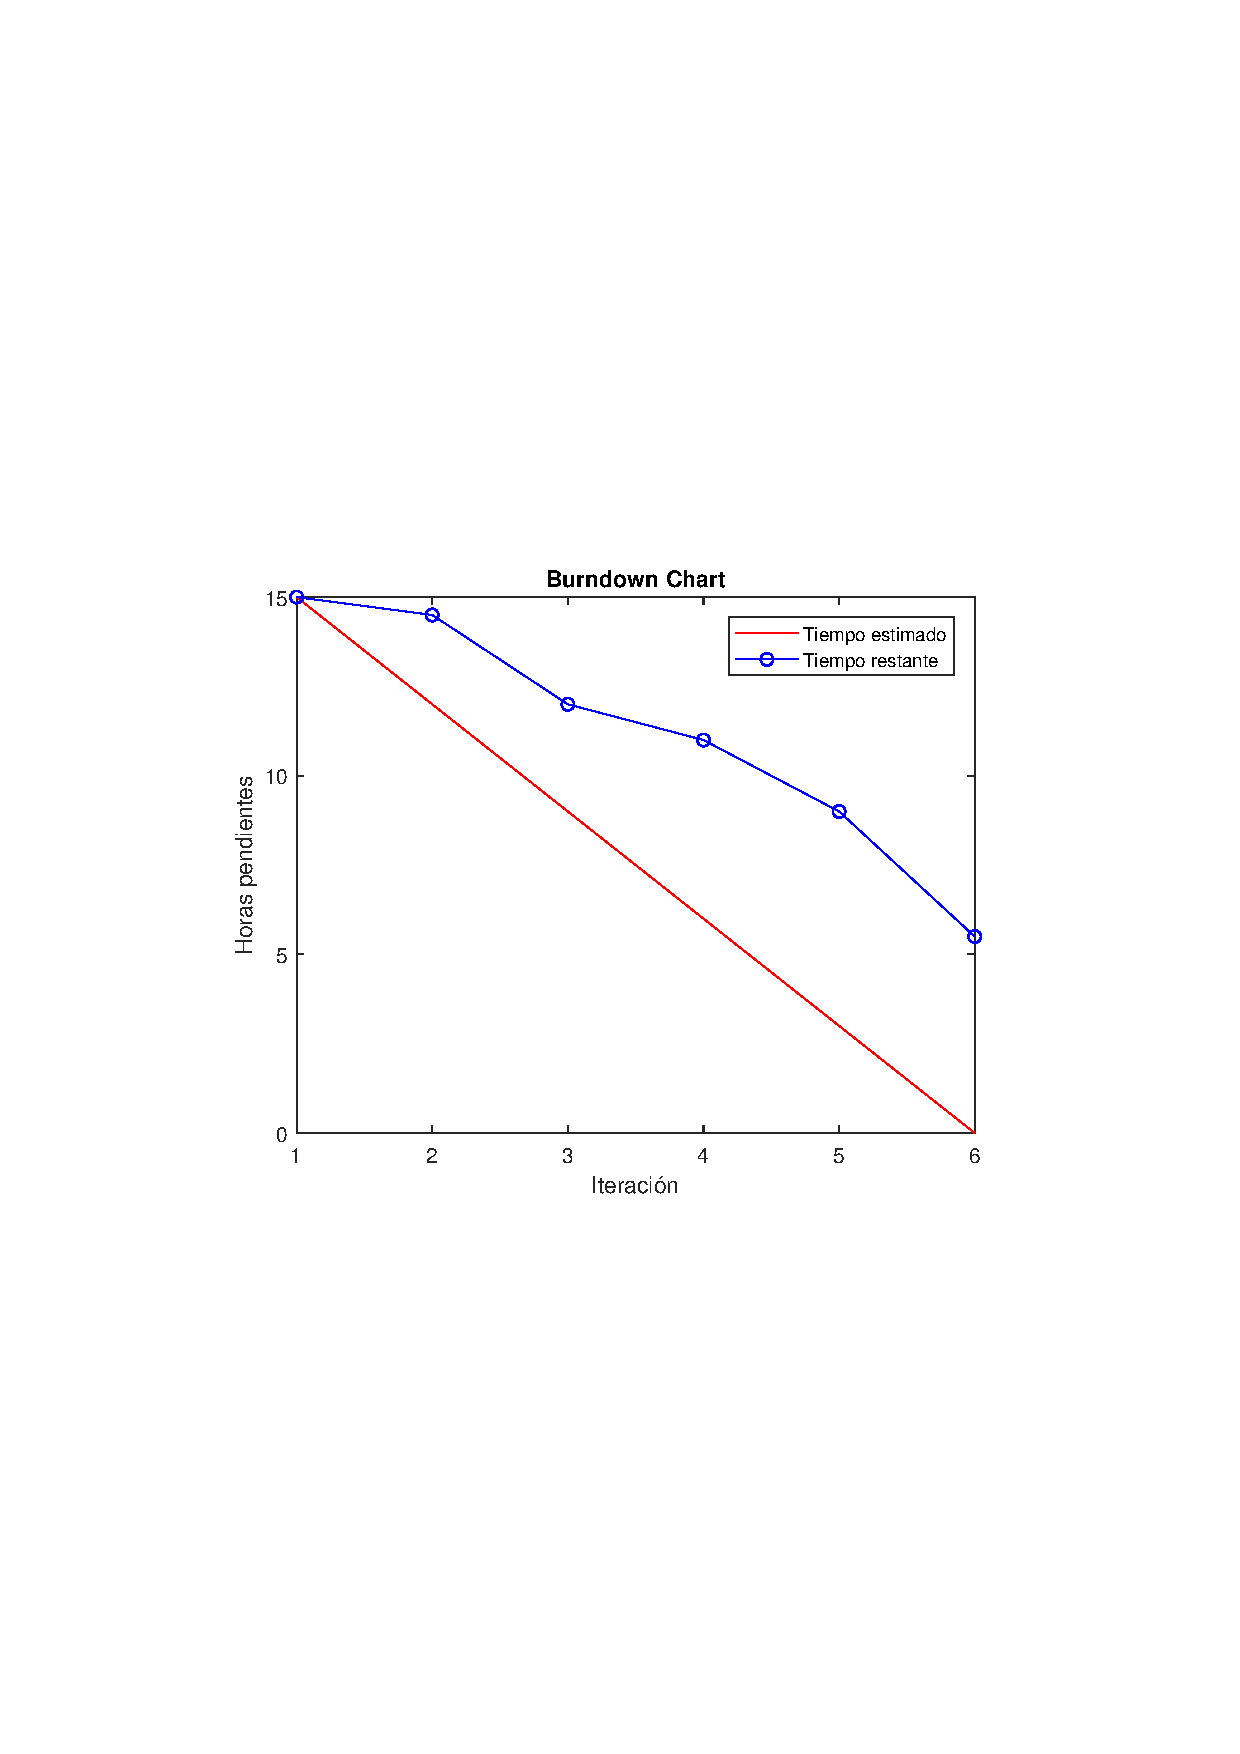
\includegraphics[width=0.85\textwidth]{burndown_chart}
	\caption{Burndown chart}
	\label{fig:burndown_chart}
\end{figure}

\newpage
\section{Código}
\subsection{alumno} \label{alumno}
\lstinputlisting{../code/alumno.hpp}
\lstinputlisting{../code/alumno.cpp}

\newpage
\subsection{baseDatos} \label{baseDatos}
\lstinputlisting{../code/basedatos.hpp}
\lstinputlisting{../code/basedatos.cpp}

\newpage
\subsection{profesor} \label{profesor}
\lstinputlisting{../code/profesor.hpp}
\lstinputlisting{../code/profesor.cpp}

\newpage
\subsection{is} \label{is}
\lstinputlisting{../code/is.hpp}

\newpage
\subsection{ppal-is} \label{ppal-is}
\lstinputlisting{../code/ppal-is.cpp}

\newpage
\section{Técnicas de validación}
En este capítulo se llevarán a cabo una serie de técnicas de validación para comprobar la corrección y completitud de la información, realizando para ello distintas matrices de validación.

\subsection{Matriz de correspondencia RF/Casos de Uso}
En la tabla \ref{tab:correspondencia_rf_cu} se muestra la matriz de correspondencia entre los requisitos funcionales y los casos de uso.

\begin{table}[h!]
	\centering
	\begin{tabular}{cccccccccc}
		\toprule
		& CU-1 & CU-2 & CU-3 & CU-4 & CU-5 & CU-6 & CU-7 & CU-8 & CU-9  \\
		\midrule
		RU-1 &  x&&&&&&&&   \\
		RU-2 &  &x&&&&&&&\\
		RU-3 &  &&x&&&&&&\\
		RU-4 &  &&&x&&&&&\\
		RF-5 &  &&&&x&&&&\\
		RF 6 &  &&&&&x&&&\\
		RU-7 &  &&&&&&x&&\\
		RU-8 &  &&&&&&&x&\\
		RU-9 &  &&&&&&&&x\\
		\bottomrule
	\end{tabular}
	\caption{\label{tab:correspondencia_rf_cu}Matriz de correspondencia RF/Casos de Uso}
\end{table}

\subsection{Matriz de correspondencia CU/Clases}
En la tabla \ref{tab:correspondencia_cu_clases} se muestra la matriz de correspondencia entre los casos de uso y las clases.
\begin{table}[h!]
	\centering
	\begin{tabular}{cccc}
		\toprule
			   & Alumno & BaseDatos & Profesor \\
		\midrule
		CU-1   & x       & x        &       \\
		CU-2   & x       & x        &       \\ 
		CU-3   & x       & x        &       \\
		CU-4   & x       & x        &       \\
		CU-5   & x       & x        &       \\
		CU-6   & x       & x        &       \\
		CU-7   & x       & x        &       \\ 
		CU-8   &         &          & x     \\
		CU-9   &         &          & x     \\
		\bottomrule
	\end{tabular}
	\caption{\label{tab:correspondencia_cu_clases}Matriz de correspondencia CU/Clases}
\end{table}